
\section{Pull request evaluation}\label{sec:pull_request_eval}
In this section, the first evaluation about pull request (PR) related to data clump refactoring is discussed. 

To ascertain the quality of refactoring, human feedback is essential. While there are metrics to evaluate whether a given refactoring is useful, the metrics do not always align with the viewpoints of developers. 

 For example, the \textit{DataClumpDoctor} tool might identify data clumps that not all developers would agree are problematic. Discrepancies might arise over the minimal number of data clump items (three in this master thesis). Additionally, developers who are  familiar with the projects's structure can more accurately judge  whether a group of variables  genuinely constitutes a data clump. In some cases, they have written the method or class themselves and have introduced the data clump on purpose because they could not find a proper name for the extracted class, or the disadvantages discussed in section \ref{sec:data_clump_not_refactor} outweigh the advantages of introducing a code smell. 

Even if developers agree that a detected data clump constitutes a data clump, there could be arguments against refactoring them. These reasons include the points  discussed in section \ref{sec:data_clump_not_refactor}. However, they could also be other reasons that apply to code smells in generals."For instance, developers might combine refactoring with the introduction of new features, rather than refactor solely for its own sake. 

As a result, collecting  the opinions and insights of developers on whether data clump refactoring is justified and can be performed by a \ac{LLM}  forms the foundation of this evaluation.

\subsection{Methodology}
In this experiment, GitHub projects are selected to refactor a selected data clump via a pull request and feedback is collected from contributors of the projects to ascertain the refactoring quality of ChatGPT. 

\subsubsection{GitHub project selection}\label{sec:github_projects}

To facilitate the evaluation, GitHub projects were selected to be analyzed in the first experiment. 


The projects are selected from the trending page of GitHub. This page list GitHub projects that have gained significant attention over a specific  period. While the exact criteria for this listing is not disclosed, popular indicators include higher-than-average forks and stars. Each selected project was evaluated based on the following criteria:
\begin{enumerate}
    \item Whether the project contains at least  10,000 \ac{LOC} of Java
        \item Whether the project  has at least 100 stars
\item Whether pull request have been merged in the last 30 days
\item Whether the project compiles and all tests run flawlessly.
\end{enumerate}

These criteria ensure the inclusion of  only larger project. This increases heuristically the chance of having a higher number of data clumps, and also the chance of getting more developers to respond to the survey as larger projects tend to be maintained by more people. 

The third criterion also influences the number of contributors and their willingness to work on the project. Only if pull request are frequently considered and closed (which does not necessarily mean that they are merged), the project is considered active enough. 

The last criterion ensures that the eventual refactoring can be evaluated smoothly. If the project does not compile properly or tests are failing, it becomes more difficult to determine whether these errors were caused by a refactoring or whether they exist from the beginning. This hinders the manual refinement step.

As a result, it is beneficial to make sure that these projects do build correctly. This can be checked by executing \textit{mvn clean package} or \textit{gradle clean build} (depending on the build system) as these commands usually run all required tests.


The total number of projects and hence pull requests were not predetermined at the beginning of the experiment. The goal was to create as many pull request as possible. 


\subsubsection{Criteria for selecting data clumps}

For each selected project, one data clump was chosen. To initialize this data clump selection process, the metrics described in section \ref{sec:data_clump_filtering} were combined. These metrics include the occurrence, size, and affected files metric. The top ten most-scored data clumps were manually reviewed to determine a data clump for refactoring. The selection process was supported by 
\begin{itemize}
\item A proposal by ChatGPT 
    \item Whether any filter discussed in section \ref{sec:data_clump_filtering} would trigger (e.~g. abstract class, generics, annotations
    \item Whether the data clump items share a common domain such that extracting a class is useful. 
    \item Whether the project is library used by other programs so that refactoring of public or protected components should be carefully scrutinized. 
\end{itemize}

All these criteria are more guidelines than strict requirements to allow flexibility.

\subsubsection{Category assignment}

After considering all of these criteria, one final data clump was selected.
After a data clump is selected, the next step is to assign the project to one of two categories to determine the extent \acs{LLM} are used to find and refactor data clumps. 



In the first category, ChatGPT performs the refactoring completely. Because transmitting whole GitHub projects would infeasible, the \textit{DataClumpDoctor} was used to detect the previously selected data clump and obtain all locations of interests. A margin of 5 was used so that 5 lines below and 5 lines above each location of interest were transmitted. 

Then, ChatGPT is instructed to refactor all data clumps in the provided locations of interest. This instruction was repeated at least ten times, in each time the context of ChatGPT was cleared so it didn't know its previous answers. 

From these ten proposal, one proposal was chosen that describes refactoring data clumps most accurately. For instance, the extracted class is valid, most usages of the data clump items are updated and all method signatures are refactored (if applicable). Generating multiple proposals is necessary because not every proposal will be correct.



The second approach for refactoring was via IntelliJ. In this case, ChatGPT only suggest a suitable name for the extracted class, but is otherwise not involved in the refactoring. Instead, IntelliJ, performs all refactoring in the manner described in section  \ref{sec:intellij_refactoring}. This results in a very consistent refactoring without any creativity. Hence, this refactoring needs only to be executed once and the first proposal can be selected immediately. 


After selecting a proposal, the proposal is applied and saved on a separate branch.
Afterwards, the proposal might not be fully correct. For instance, there might none-updated method calls, missing semicolons etc. An additional problem occurs if codestyle tools like SpotBugs or Checkstyle are employed. If the refactoring by the \ac{LLM} does not conform to the required codestyle, the code might not compile because the developers of the project force a certain style. Therefore, a manual correction step is performed. The project is  manually changed in such a way that it fully compiles. However, no creative refactoring is performed. For instance, if one part of the source code was not refactored, it was refactored like another part regardless of whether another refactoring might have make more sense. This reduces human intervention to a minimum and ensures that the creative part of the refactoring is done by the \ac{LLM}. 

As soon as this manual refactoring finished and the program compiles, the changes were squashed into one commit and a pull request was created in the respective repository. In this pull request, the maintainers were described the purpose of this pull request and  the definition of data clumps used in this master thesis. They were asked to give feedback by filling out a feedback form or by giving feedback via GitHub comments under the respective pull request. It was explicitly stressed that rejecting the pull request would not be perceived negatively. 

"Feedback from both the form and comments was collected and evaluated as described in 
 section \ref{sec:feedback_survey}

\subsubsection{Feedback survey}\label{sec:feedback_survey}

Feedback is collected from two sources that are available on each pull request. 

One  natural way of providing feedback over GitHub is via comments. These comment can be review comments that address specific parts of the code or general comments unrelated to any code that addresses the pull request as a whole. \cite{10.1145/3597208}. Therefore it is an important source of determining the acceptance of the proposed refactoring. However, since the comments are natural texts, the evaluation is more challenging.


On the other hand, the likert scale is a common method in surveys. It consists of statements that claim a certain fact and the respondents have to express their opinion to each statement by choosing one discrete attitude category per statement . \cite{edmondson2005likert}

For instance, a statement might be \enquote{refactoring data clumps is useful}, and the list of available attitudes might be
\begin{itemize}
    \item Strongly agree
    \item Agree
    \item Neutral
    \item Disagree
    \item Strongly disagree
\end{itemize}

Using the method evaluating the variance of opinion can be eased as the possible answers are discrete and easy to map on a numerical scale (e.~g. 0 for strongly disagree to 5 for strongly agree). These values can be used in statistical analysis (e.~g. arithmetic mean) to describe tendencies. However, it should be noted that such an analysis has its flaws as it implies that the distance between response categories is constant.For instance, choosing between \enquote{strongly disagree} and \enquote{disagree} might be simpler or more complex than deciding between \endquote{strongly agree} and '\enquote{agree} \cite{HARPE2015836}


For this master thesis, the survey platform \textit{lamapoll} \cite{lamapoll} was used.  The following statements should be addressed by the respondents:
\begin{enumerate}
\item Data clumps are a code smell that should be fixed.
\item Using LLMs in software development can be helpful to improve code quality.
\item The proposed refactoring maintains or improves the quality of the code.
\item The proposed refactoring has  adequately identified and preserved the original functionality and intent of the code.
\item The name of the new extracted class(es), fields and methods are well-chosen.
 \item The location of the extracted class(es) are well-chosen.
 \item For how long have you been contributing to this project?
\item For how long have you been a developer in Java ? 
\item Please input the URL of the GitHub project from where you got to this survey.

\end{enumerate}


The statements 7--9 are actually questions that do not use the likert scale. Question 7 attempts to assess the experience of the developer about this project. Question 8 similarly is aimed to obtain the programming experience of the respondent in the Java language.

The purpose of question 9 is to create a connection between the survey and the pull request of the project as the survey platform does not allow such a link easily.

The full text of the pull request can be found in appendix \ref{app:pr_text}.


\subsubsection{Evaluation metrics}

For the evaluation, the following metrics are used:
\begin{description}
    \item [Acceptance rate] How many PRs are merged or rejected.
    \item [Likert scale] The numerical value of the likert scale.
    \item[Discrete review subjects] These are topics mentioned in the comments that are either positive or negative. For instance, a comment might mention that the readability is improved or worsened by a refactoring. The occurrence of these topics can be counted.   Table \ref{tbl:feedback_categories} explains the most important feedback categories. 

\end{description}

By grouping the pull requests into categories (e.~g. by refactoring method, data clump type etc.), these metrics can be used to gather hindsight into the acceptance of \ac{LLM}-assisted refactoring. 


\begin{table}
\begin{tabular}{p{2cm}|p{10cm}}
	Comment & Description\\\hline
	\textit{Refactoring not worth it} & The refactoring does not provide enough advantages to justify it\\\hline
	\textit{Readability} & The readability of the source code is reduced \\\hline
	\textit{Not enough} & While the refactoring could be a good idea, more changes should be performed to make the refactoring more useful \\\hline
	\textit{Intentional design choice} & The duplication of variables is warranted so that changes are unnecessary \\\hline
	\textit{Style adaption} & The refactored code does not fit into the rest of the code as it violates style guidelines. \\\hline
	\textit{Complexity} & The refactoring introduces more complexity\\\hline
	\textit{Semantic changes} &  The refactoring changes the semantic of the code\\\hline
	\textit{Performance}& The performance implications of the refactoring are too grave \\\hline
	\textit{Java record better} & the extracted class suggested by the refactoring could be converted into a Java record \\\hline
	\textit{Extracted class should not be public} & Instead of creating a new file for an extracted class, it should be located inside another class and does not need to be public \\\hline
	
\end{tabular}
\caption{Feedback categories explained}
\label{tbl:feedback_categories}
\end{table} 


\subsubsection{Threats to validity}

The survey evaluation has some threats to its validity that should not be disregarded.

To begin with, the selection of GitHub project is not completely unbiased. For instance, currently trending GitHub projects were chosen although it is not certain why they were popular. Therefore, the maintainers of the project might not be fully prepared to deal with associated surge in pull requests associated with trending projects. This can increase the chance that a pull request (even though reasonable and well-meant) is summarily rejected. \cite{10.1145/3366423.3380272}

Additionally, only projects that do build flawlessly were considered. Usually, this should be case for every project, but the reality differs. For instance, the operating system, the installed libraries, the Java version, and other components can have a significant impact on whether all unit tests complete without errors and the project builds.  While every effort was made to give each project a chance to compile, at some point, time constraints prevented endless consideration of a project. Hence, if even after testing on multiple system, reading the associated documentation, and testing multiple Java version, no fully functional build was achieved, the project was disregarded.

It is also important to consider the manual correction process, as it could introduce mistakes or bugs due to human error rather than errors from the \ac{LLM}. Feedback regarding these errors must be filtered out as they are not relevant. 


Additionally, the decision to accept or reject a pull request can depend on many factors. For instance, the current mood of participating developers can influence the rejection rate \cite{detecting_emotional}.

For larger project, bureaucracy was also a factor that prevented the creation of pull requests. For instance, some projects require that pull request must always relate to an existing issue so that the general idea can be discussed without providing source code. For usual contributors, this might be beneficial as they do not need to spend time on writing code that is rejected in the end because the developers do not like the general approach. For the purpose of this evaluation, the actual source generated is essential, so creating an issue first would be possible,  but more burdensome  and would not add much value. Nevertheless, the sole existence of such rules was not a criterion to filter out a project. 

\subsubsection{Ethical consideration}
As this survey contains interaction with human-beings, a small analysis on the ethical implications is conducted. Several precautions are undertaken to address any possible ethical concern. 

First of all, full transparency is provided  with regard to the pull request. The pull request message explicitly states the purpose of the PR as a part of a scientific project. Also the use of an \ac{LLM} is explicitly stressed so that no misunderstanding can occur. However, the participants are not aware of the extent \acp{LLM} have been used and do not know which model was used. Such details have however been revealed during discussion of the PR if further feedback from new participants was unlikely.

Additionally, the requests were not sent en masse but after careful consideration. Only if it is thought that a pull request does compile, passes all unit test and otherwise does not have major issues, the pull request is submitted. Of course, mistakes can happen so that this approach cannot guarantee hundred percent fault-free code. Since many projects needs to be considered, the extensive knowledge of the software project, which a regular contributor has, is missing, so that the chance of faults are higher. Nevertheless, pull requests can be created by anyone and the review process by continuous integration and deployment tools and human beings is a safeguard to limit the risk of faulty code added to the code base. 

Last but not least, it was attempted to minimize the burden on the reviewers. For instance, data clumps affecting a significant number of files were not refactored. Also only one pull request per project was created, thereby minimizing the chance that a participant might review multiple pull requests. \footnote{At one instance, an ethical complaint was filled because of the use of \acp{LLM} and the perceived spamming of pull requests. This complaint was however dismissed by the competent organizations of the University of Osnabrück}.  


\subsection{Results}

At the conclusion of this experiment, pull requests to 40 projects have been submitted. Of those 40 projects,  feedback for 31 projects could be obtained. In the remaining 9 cases, either the pull request is still open, was closed without meaningful feedback or merged without meaningful feedback. In 8 cases, the pull request was eventually merged which indicates a acceptance rate of twenty percent. 

In 7 projects, feedback was provided via the survey. Figure \ref{fig:boxplot_survey} shows the result of the evaluation if only the likert scores are considered. 

The boxplot shows that data clumps are considered as a code smell worth to fix. It can also be that \ac{LLM} are considered to be a valuable tool in software development and can help to improve the software quality.

The concrete refactoring however however was received with mixed feelings. While the names and locations of the extracted classes, fields, and methods are favorably rated, there is a notable opposition to the claim that the proposed refactoring improves or at least maintains the quality of the code. Also, while there is agreement that the functionality of the code is preserved, the likert value shows more disagreement.

\begin{figure}
    \centering
    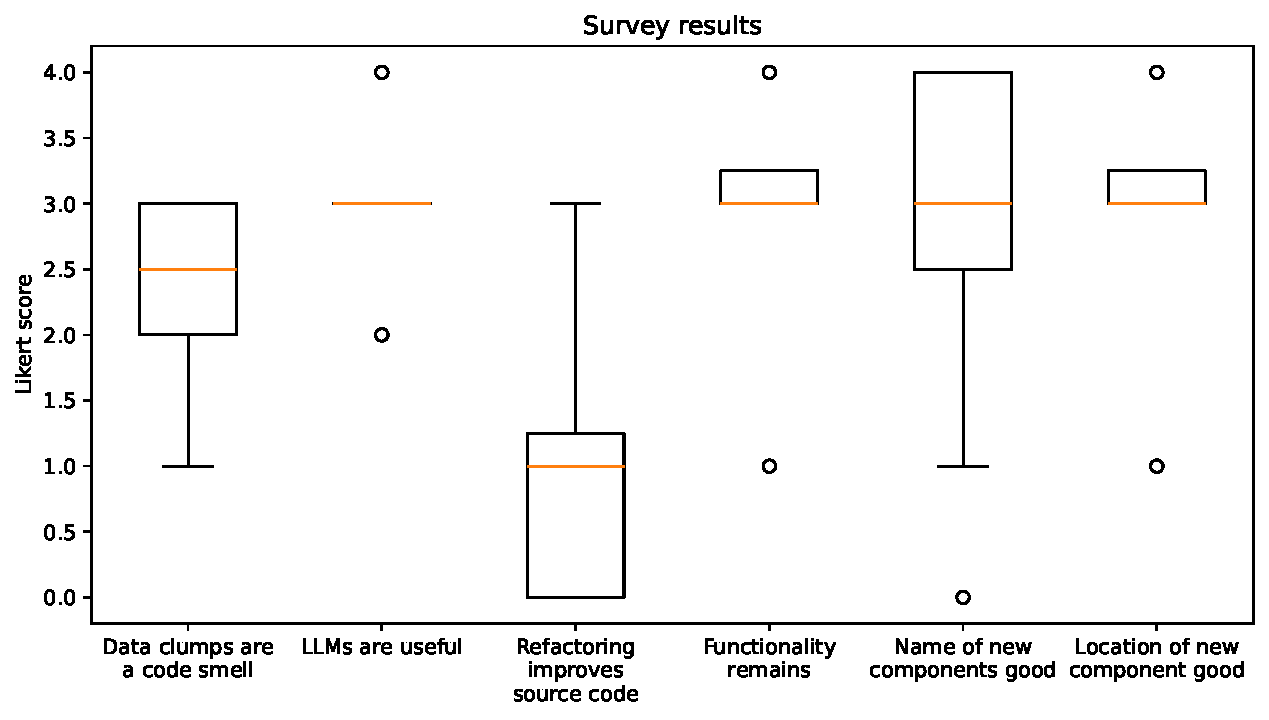
\includegraphics[width=\columnwidth]{figures/chapter5/survey_results.pdf}
    \caption{Boxplot of Likert score from survey}
    \label{fig:boxplot_survey}
\end{figure}


The textual feedback contains further hindsight on why the refactoring was perceived more negatively. In six instances, the reviewers increases a perceived increase of complexity. In 11 instances, there are concerns about the readability. Also performance concerns are common as the refactoring entails creating new instances. This criticism was shared five times. Another argument that was made nine times is that the refactoring is not worth it as the developers see no obvious benefit in refactoring this data clump.

The difference of the feedback between the traditional refactoring and the \ac{LLM}-driven refactoring is slim. However, there are noteworthy observations. For instance, the traditional approach receives four instances where the maintainers are dissatisfied with style adaption of  the code. This means that the refactored code does not fit into the rest of the code. This point was not risen for the \ac{LLM}-generated code. 

Also, in general, criticism about the code readability is raised more for the project refactored using the traditional approach than the \ac{LLM}-based approach.

Comparing the refactoring of fields-to-fields to parameters-to-parameters data clump, there are also some differences. The readability of refactored fields-to-fields data clump was is scored more negatively than that of parameters-to-parameters data clump. Also the adoption of the code to the style is criticized more if fields-to-fields data clump are refactored. Additionally, more meaningful comments were received for parameters-to-parameters data clump.

Noteworthy, the refactoring performed by the model has not always refactored an actual data clump as defined in section \ref{sec:data_clump_def}. In one case, a group of fields that only existed in one class but have a semantic relationship were extracted to a class. Nevertheless this pull request was merged indicating that a close semantic connection of variables can warrant refactoring. However, in two other similar cases, the pull request was rejected. 

The occurrence of a data clump strongly influences the likelihood of a refactoring being merged. Refactorings that were not merged had a mean occurrence of 4.5, whereas those that were merged had a mean occurrence of 10.7

If one considers the size of the refactored data clump, there are also some patterns. For instance, the respondent believe that larger data clumps reduce the complexity. However, on the other hand, the readability of the refactored source ode was higher if the data clump is smaller.



\subsection{Discussion}
The results shows that surveys via GitHub pull request pose some challenges. Some pull requests are left unanswered, while others are closed without comments or the comment contains very general feedback and not helpful for evaluating the survey. Additionally, the tendency of developers to use GitHub for giving feedback  instead of the suggested survey platform complicates a solid analysis of the evaluation.

One main finding on the evaluation results is the importance of selecting suitable data clumps for refactoring. In many cases, the developers believe that the suggested refactoring is not worth it, makes the code harder to read or the performance implication are too negative. This shows that data clumps are a code smell where there is a wide disagreement on when refactoring is warranted and when not. because all tested projects have a multitude of different data clumps that have various sizes, affected files or included variables, it is very difficult to select a suitable data clump. Traditional metrics like the size or the occurrence seem to have only a weak influence on the acceptance of data clump refactoring. Instead, the relationship of the variables is more often a better indicator. Here, the model can be a great help as it does not necessarily rely on these common metrics. However, as it can bee seen, the choice by the model is often not enough. Instead, the inherent knowledge of the contributors of a project is a major factor to decide whether refactoring is warranted. Only with information about the scope, goals, and issues of a project, it is possible to determine where refactoring is more likely to be warranted. Even with the help of \ac{LLM}, external contributions can hardly mitigate this lack of knowledge which explains many pull request rejections. 

Another highlighted issue is the legal implication of using \acp{LLM} which is a significant concern for open source developers. Because large language models derive their knowledge from a multitude of sources, cannot give these sources adequately and are relatively new, the developers are too cautious to integrate refactorings by \acp{LLM}."Even without knowing that a traditional approach was used for the actual refactoring, merely mentioning the use of LLMs led to rejections.  This indicates that the legal implication of these models are fundamental and needs to be resolved before they can be accepted. 